\documentclass[11pt, a4paper]{article}

\usepackage[top = 0.7 in, bottom = 0.7 in, left = 0.7 in, right = 0.7 in ]{geometry}

\usepackage{amsmath, amssymb, amsfonts}
\usepackage{enumerate}
\usepackage{array}
\usepackage{multirow}
\usepackage{dingbat}
\usepackage{fontawesome5}
\usepackage{tasks}
\usepackage{bbding}
\usepackage{xcolor}
\usepackage{graphicx}
\usepackage{hyperref}

\definecolor{col1}{HTML}{e75e05}
\definecolor{col2}{HTML}{d30bb1}

\title{MSMS - 105}
\author{Ananda Biswas}
\date{}


\begin{document}

\maketitle

\begin{center}
\textbf{Assignment 03}
\end{center}


\OrnamentDiamondSolid \hspace{0.5cm} \textcolor{blue}{\textbf{Objective :}} To visuallly illustrate the concept of \textbf{Statistical Regularity} through an example. \\

\faArrowAltCircleRight[regular] \textcolor{col1}{\textbf{\textit{Theory}}} : Statistics deals with random experiments. We may think of randomness as ``irregularity". However, in certain situations, even outcomes of random experiments show a regularity that is similar to deterministic behaviour. This is called Statistical Regularity. \\

\hspace{1cm} In the following we shall consider a mathematical version of Ludo and see how a \textit{deterministic behaviour} shapes out of many trials of a random experiment.  \\


\hspace{0.5cm} Assume $\mathbb{R}^2$ as our Ludo board and consider a die with 4 equally likely outcomes. We start our game with $(x, y) = (0, 0)$. We toss the die and update $(x, y)$ as per the following rules.

\begin{table}[!htbp]
\def\arraystretch{1.5}

\begin{center}
\begin{tabular}{|>{\centering}m{2cm}||>{\centering\arraybackslash}m{8cm}|}

\hline

Die result & New $(x, y)$ \\

\hline
\hline

1 & $(0.8x + 0.1, 0.8y + 0.04)$ \\

2 & $(0.5x + 0.25, 0.5y + 0.4)$ \\

3 & $(0.355(x - y) + 0.266, 0.355(x+y) + 0.078)$ \\

4 & $(0.355(x + y) + 0.378, 0.355(y-x) + 0.434)$ \\

\hline

\end{tabular}
\end{center}
\end{table}

On getting new $(x, y)$, we plot it on $\mathbb{R}^2$. \\

\faArrowAltCircleRight[regular] \textcolor{col1}{\textbf{\textit{Visualization}}} : \href{https://github.com/sakunisgithub/R-programming/blob/master/msc_sem_1_practicals/mahaveer_sir_assignments/assignment_03/assignment_03.R}{\textcolor{blue}{\textbf{Program to create the following animation is here.}}} \\

After playing the game for $n = 10$ times, we get the following scatter of points - just 10 random points with no visible pattern.

\begin{figure}[h]
\centering
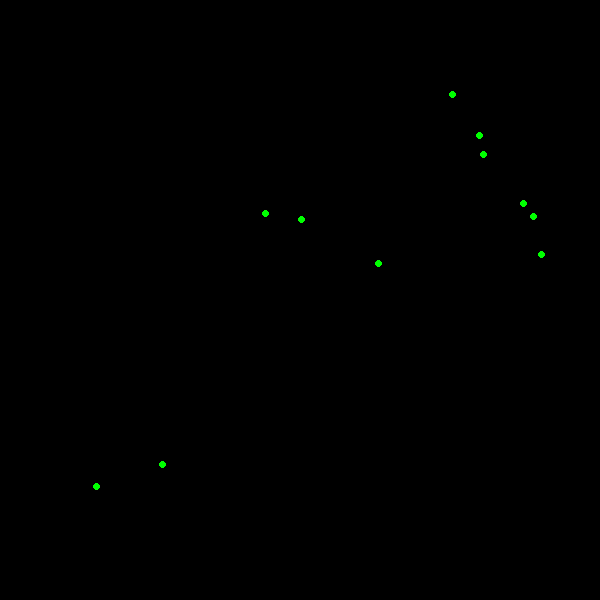
\includegraphics[scale=0.3]{01}
\end{figure}

\newpage

For $n = 100$, we get

\begin{figure}[!htbp]
\centering
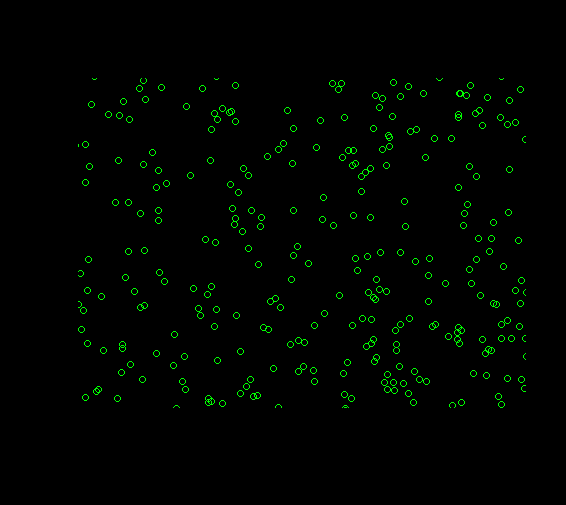
\includegraphics[scale=0.3]{02}
\end{figure}


For $n = 500$, we get

\begin{figure}[h]
\centering
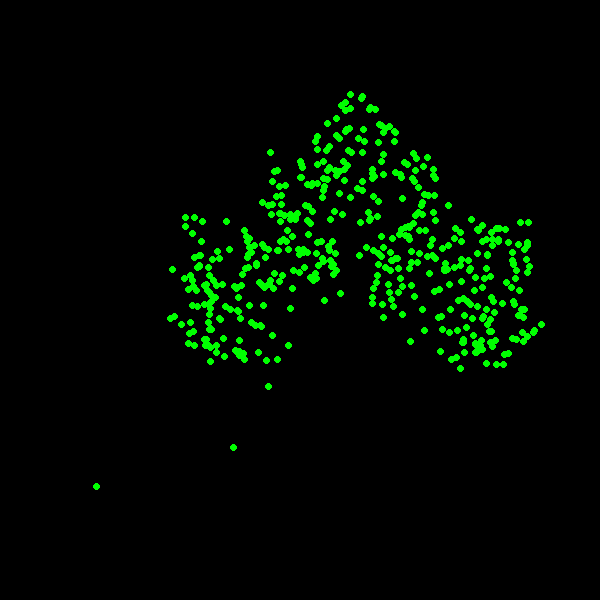
\includegraphics[scale=0.3]{03}
\end{figure}


For $n = 1000$, we get

\begin{figure}[h]
\centering
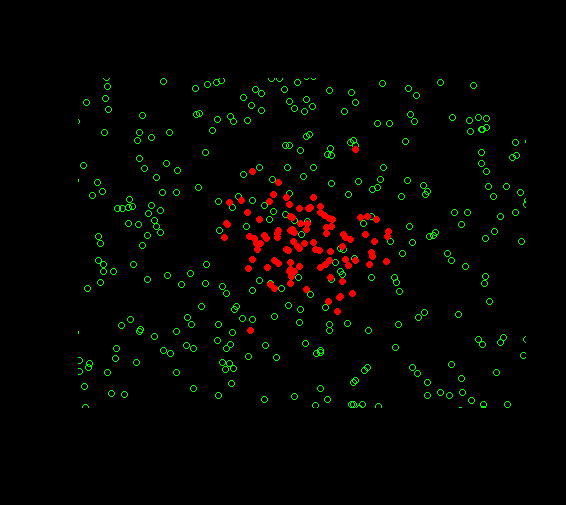
\includegraphics[scale=0.3]{04}
\end{figure}

A certain cluster of points seems to be getting prominent gradually. \\

For $n = 5000$, we get

\begin{figure}[!htbp]
\centering
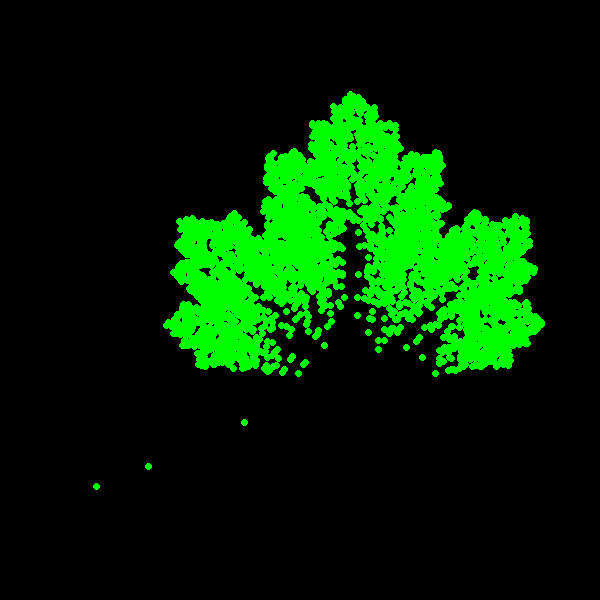
\includegraphics[scale=0.3]{05}
\end{figure}

All these random points together create a leaf.

\newpage

Notice that, all these 5000 points random points. But together they create a deterministic shape like a leaf. If we again play the game 5000 times, we shall get a new plot as below.

\begin{figure}[h]
\centering
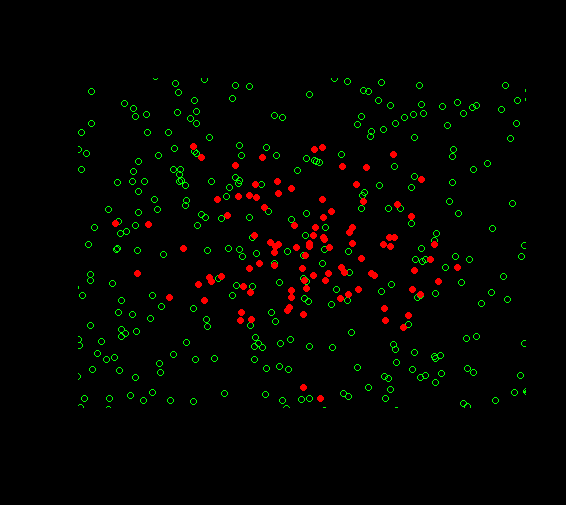
\includegraphics[scale=0.3]{06}
\end{figure}

The new 5000 points are another set of random points, hardly similar with previous 5000 points. But they create the same scatter of points exactly identical as before. This phenomenon of getting a deterministic behaviour out of randomness is called \textbf{Statistical Regularity}. \\

\hspace{0.5cm} Leaves of plants, fingerprints on hands are great examples how statistical regularity is part and parcel of nature.


%
%\begin{table}[h]
%
%\begin{center}
%\begin{tabular}{ccc}
%
%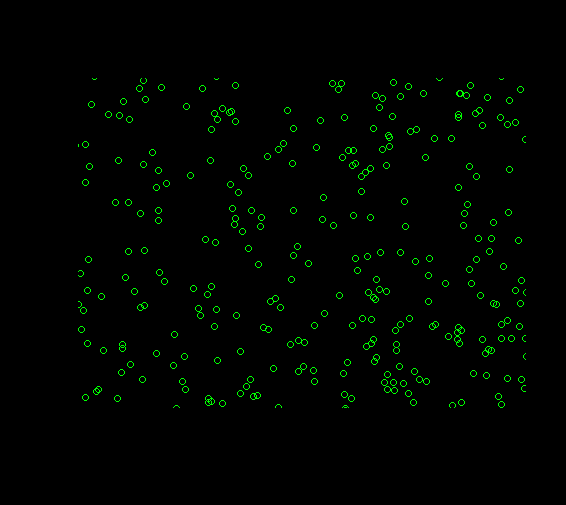
\includegraphics[scale=0.2]{02} & 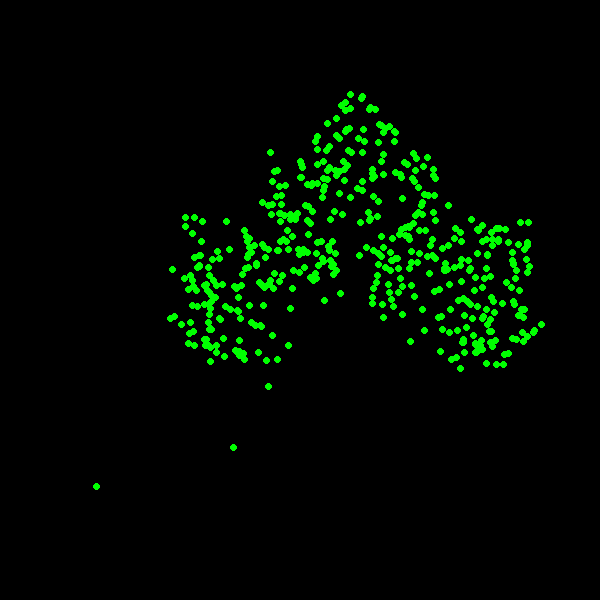
\includegraphics[scale=0.2]{03} & 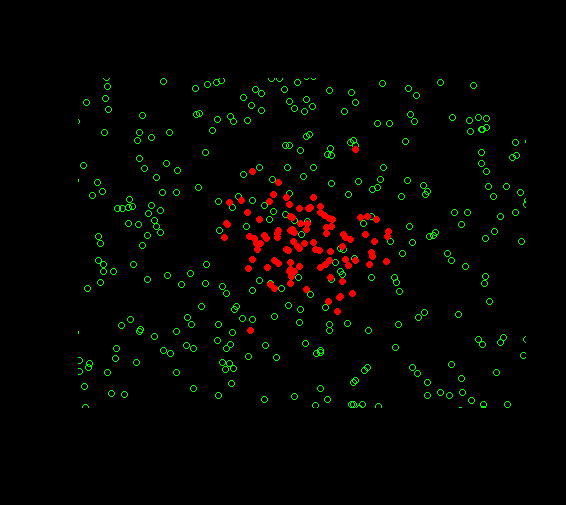
\includegraphics[scale=0.2]{04} 
%
%\end{tabular}
%\end{center}
%\end{table}
%
%\newpage
%
%\begin{table}[h]
%
%\begin{center}
%\begin{tabular}{cc}
%
%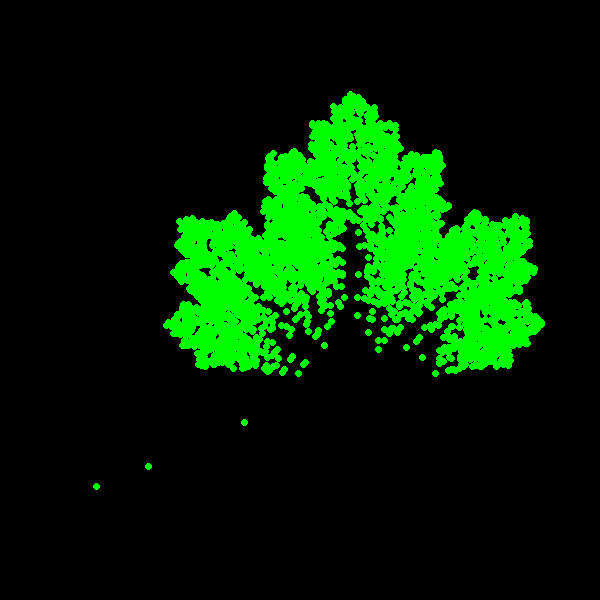
\includegraphics[scale=0.2]{05} & 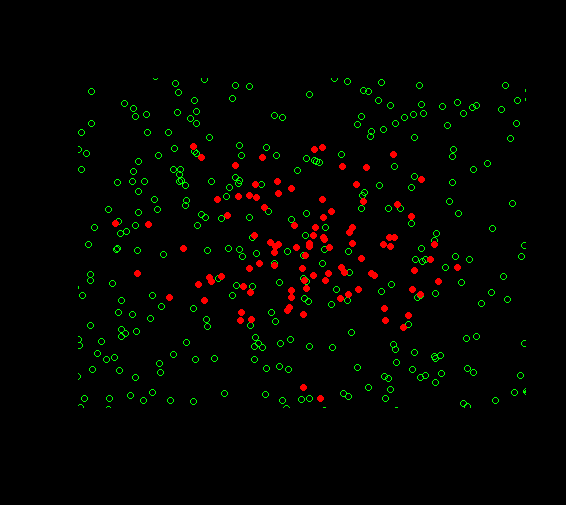
\includegraphics[scale=0.2]{06} 
%
%\end{tabular}
%\end{center}
%\end{table}
%
%
%\smallpencil \hspace{0.2cm} \textcolor{col2}{\textbf{\textit{Rotating}}} : Pre-multiplying any vector $ \begin{bmatrix} a \\ b \end{bmatrix} $ $\in$ $\mathbb{R}^2$ by 
%  $ \begin{bmatrix} 
%      \cos \theta & - \sin \theta \\
%      \sin \theta & \cos \theta
%    \end{bmatrix} $ rotates the vector by an angle $\theta$ anti-clockwise. Here we take $\theta = \dfrac{\pi}{4}$ and rotate the above vectors by $45^{\circ}$ anti-clockwise. \\
%    
%\faArrowAltCircleRight[regular] \textcolor{col1}{\textbf{\textit{Visualization}}} : \href{https://github.com/sakunisgithub/R-programming/blob/master/msc_sem_1_practicals/mahaveer_sir_assignments/assignment_04/transformation_3.R}{\textcolor{blue}{\textbf{Program to create the following animation is here.}}}
%
%\begin{table}[h]
%
%\begin{center}
%\begin{tabular}{ccc}
%
%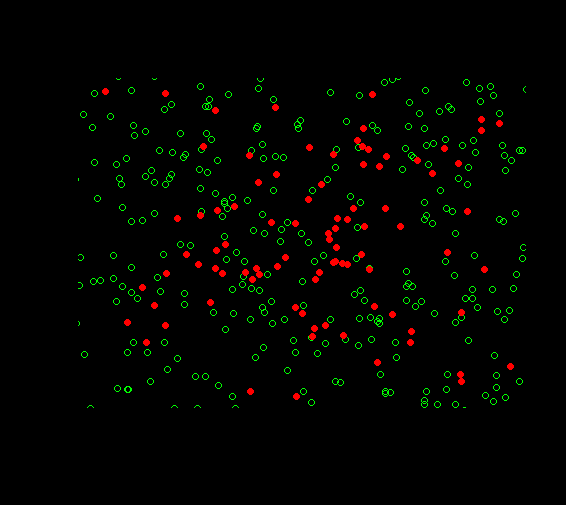
\includegraphics[scale=0.2]{07} & 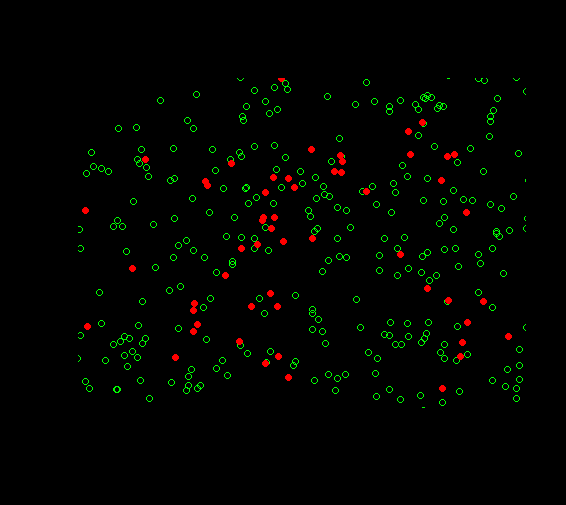
\includegraphics[scale=0.2]{08} & 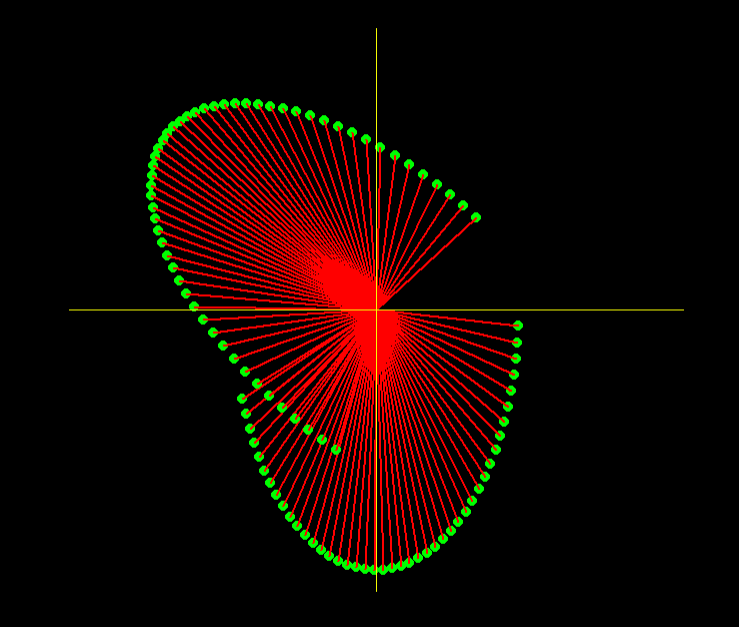
\includegraphics[scale=0.2]{09} 
%
%\end{tabular}
%\end{center}
%\end{table}
%
%\begin{table}[h]
%
%\begin{center}
%\begin{tabular}{cc}
%
%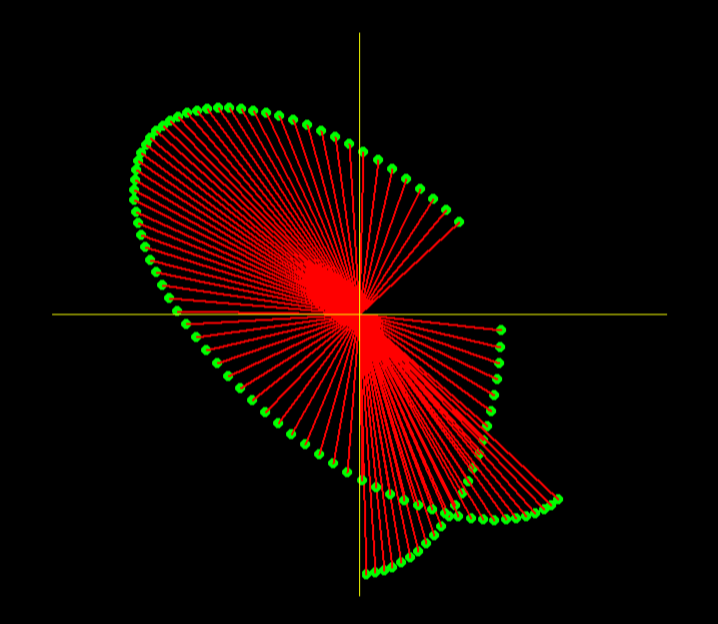
\includegraphics[scale=0.2]{10} & 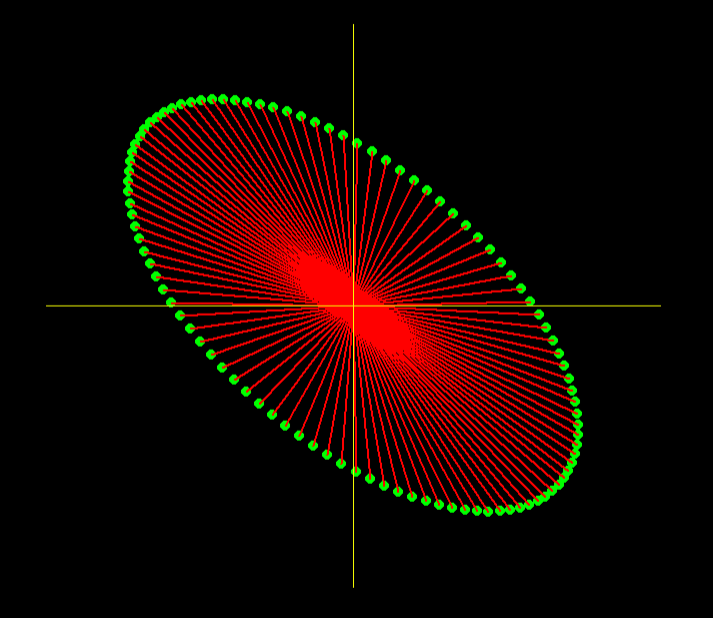
\includegraphics[scale=0.2]{11} 
%
%\end{tabular}
%\end{center}
%\end{table}
%
%
%\smallpencil \hspace{0.2cm} \textcolor{col2}{\textbf{\textit{Composition of Transformation}}} : Multiplication of two matrices results in a matrix that represents the combination of their transformations. Above we first stretched the 100 vectors two times along $y-$axis and then rotated them $45^{\circ}$ anti-clockwise. We can achieve the same by just pre-multiplying all the vectors by
%	\begin{gather*} 
%	  \begin{bmatrix} 
%      	\cos \theta & - \sin \theta \\
%	      \sin \theta & \cos \theta
%    	  \end{bmatrix}_{\theta = \dfrac{\pi}{4}}
%    	  	 \cdot 
%	  \begin{bmatrix} 
%	      1 & 0 \\
%      	0 & 2 
%        \end{bmatrix}         
%        =         
%        \begin{bmatrix}
%        	0.7071068 & -1.414214 \\
%        	0.7071068 & 1.414214
%        \end{bmatrix}
%      \end{gather*}
%
%\faArrowAltCircleRight[regular] \textcolor{col1}{\textbf{\textit{Visualization}}} : \href{https://github.com/sakunisgithub/R-programming/blob/master/msc_sem_1_practicals/mahaveer_sir_assignments/assignment_04/transformation_4.R}{\textcolor{blue}{\textbf{Program to create the following animation is here.}}}
%
%\begin{table}[!htbp]
%
%\begin{center}
%\begin{tabular}{ccc}
%
%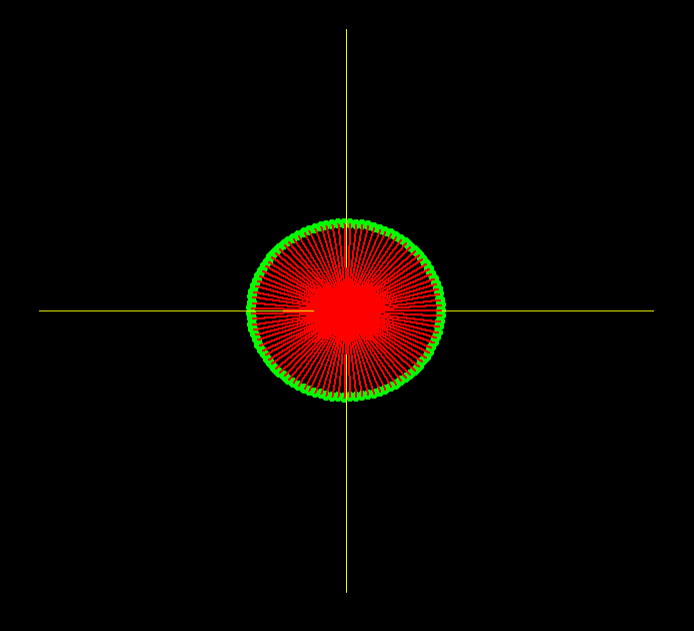
\includegraphics[scale=0.2]{12} & 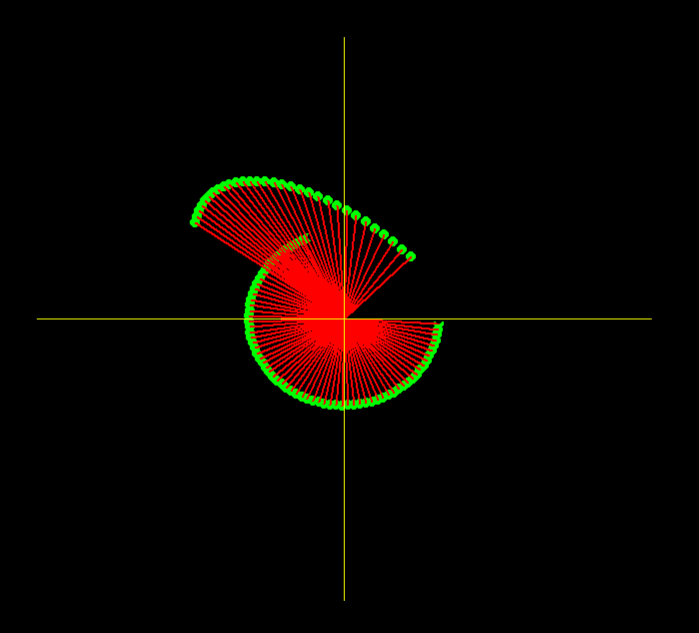
\includegraphics[scale=0.2]{13} & 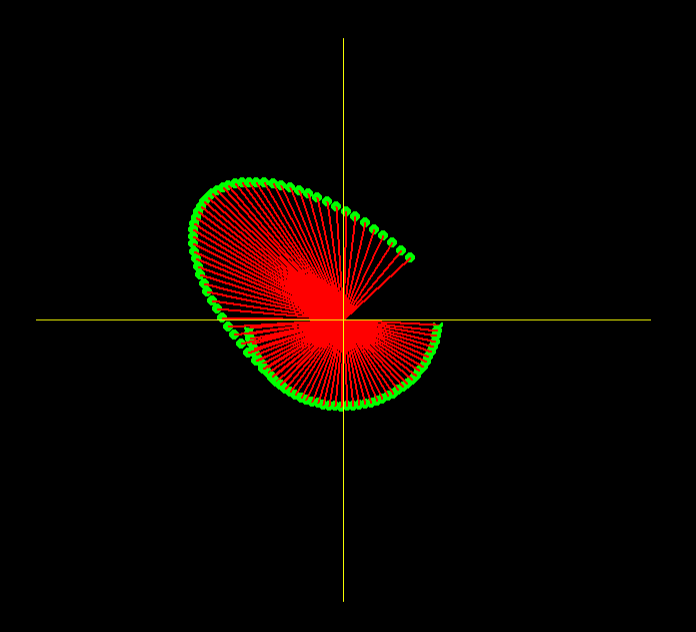
\includegraphics[scale=0.2]{14} 
%
%\end{tabular}
%\end{center}
%\end{table}
%
%\newpage
%
%\begin{table}[h]
%
%\begin{center}
%\begin{tabular}{cc}
%
%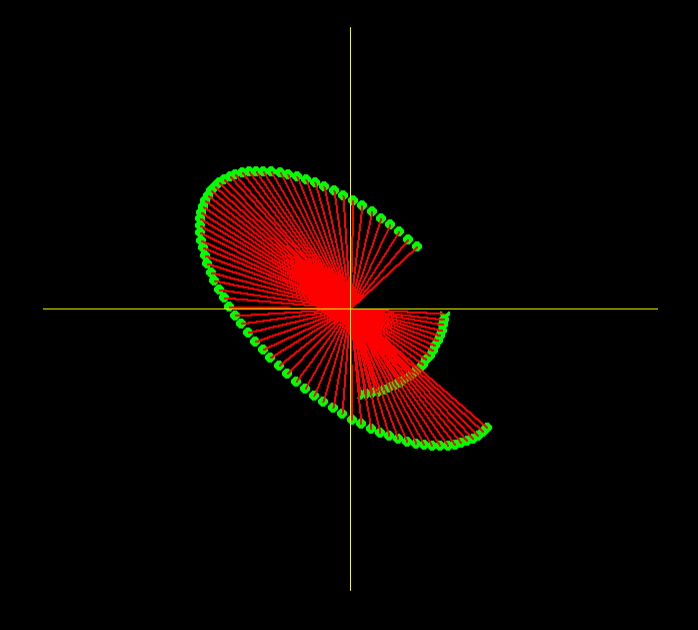
\includegraphics[scale=0.2]{15} & 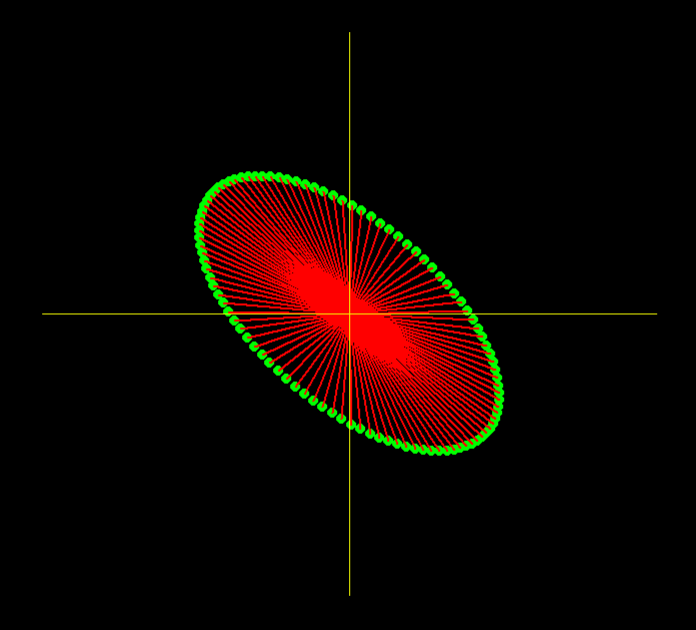
\includegraphics[scale=0.2]{16} 
%
%\end{tabular}
%\end{center}
%\end{table}
%
%
%\smallpencil \hspace{0.2cm} \textcolor{col2}{\textbf{\textit{Vector Spaces and Dimension}}} : Multiplying all the vectors of a vector space by a matrix of rank $r$ creates a new vector space of dimension $r$. Here we pre-multiply all the 100 vectors by 
%	$ \begin{bmatrix} 
%		1 & 1 \\
%		1 & 1
%	\end{bmatrix} $ which has rank 1 and see how $\mathbb{R}^2$ reduces to a straight line only. \\
%	
%\faArrowAltCircleRight[regular] \textcolor{col1}{\textbf{\textit{Visualization}}} : \href{https://github.com/sakunisgithub/R-programming/blob/master/msc_sem_1_practicals/mahaveer_sir_assignments/assignment_04/transformation_5.R}{\textcolor{blue}{\textbf{Program to create the following animation is here.}}}
%
%\begin{table}[!htbp]
%
%\begin{center}
%\begin{tabular}{ccc}
%
%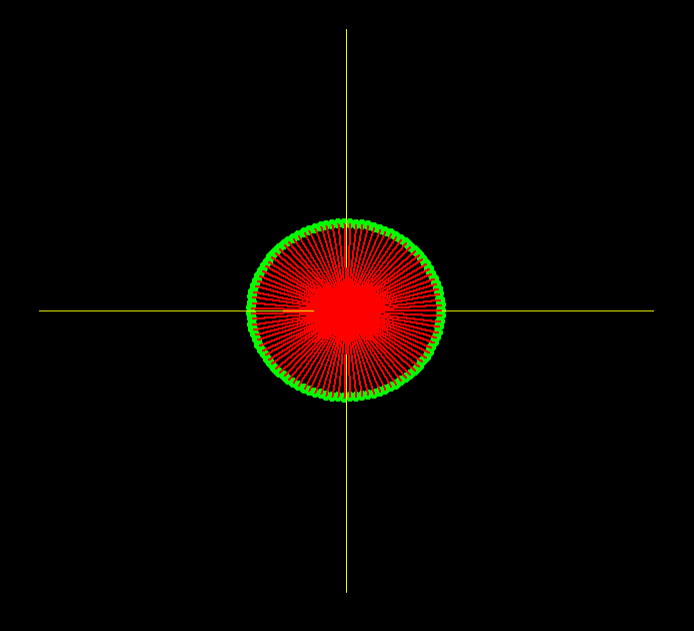
\includegraphics[scale=0.2]{17} & 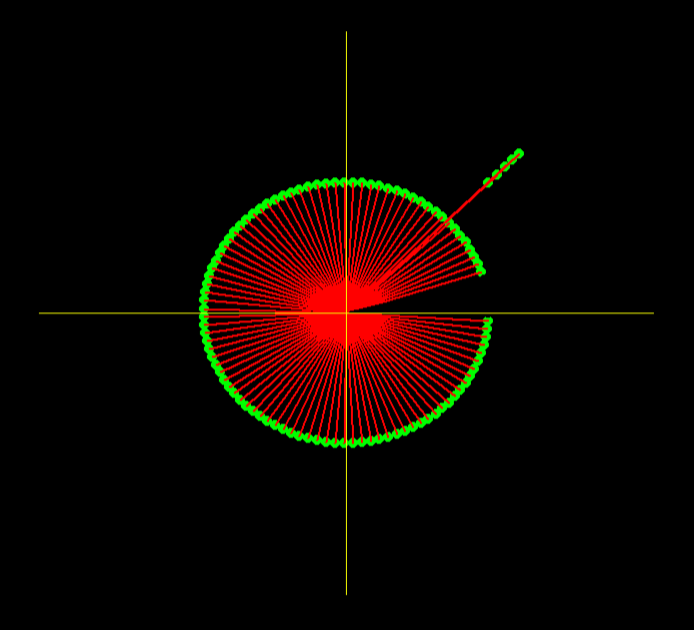
\includegraphics[scale=0.2]{18} & 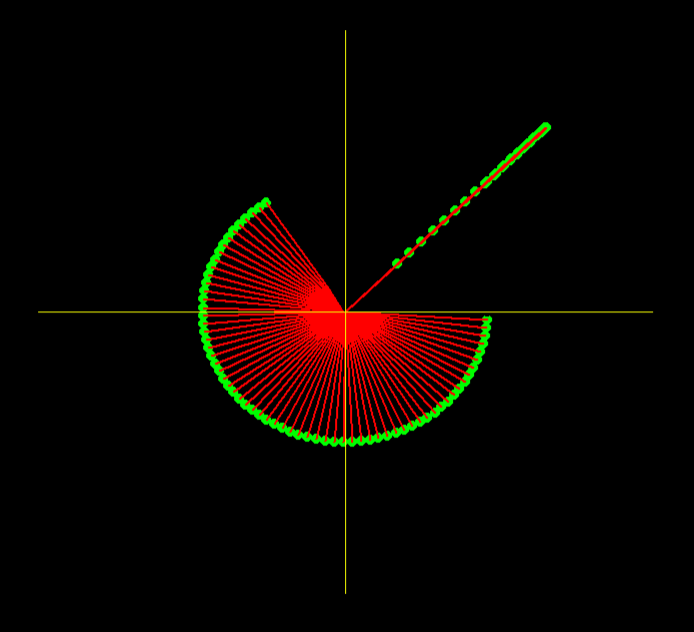
\includegraphics[scale=0.2]{19} \\
%
%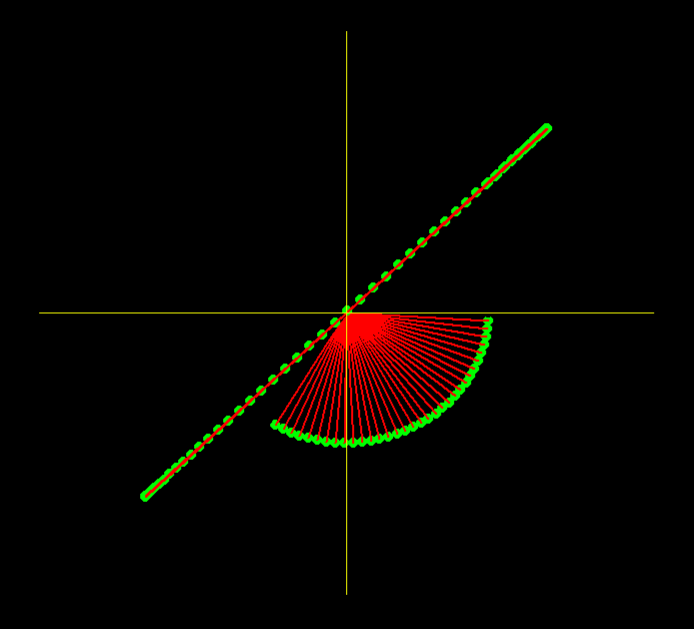
\includegraphics[scale=0.2]{20} & 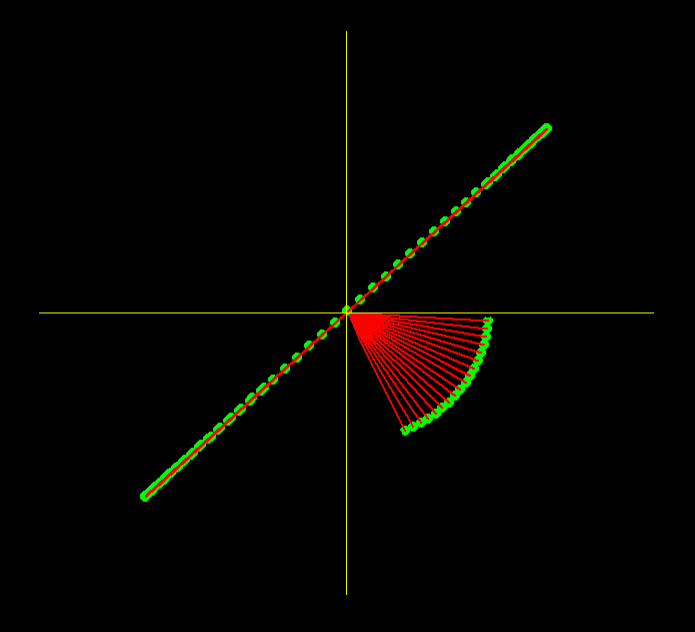
\includegraphics[scale=0.2]{21} & 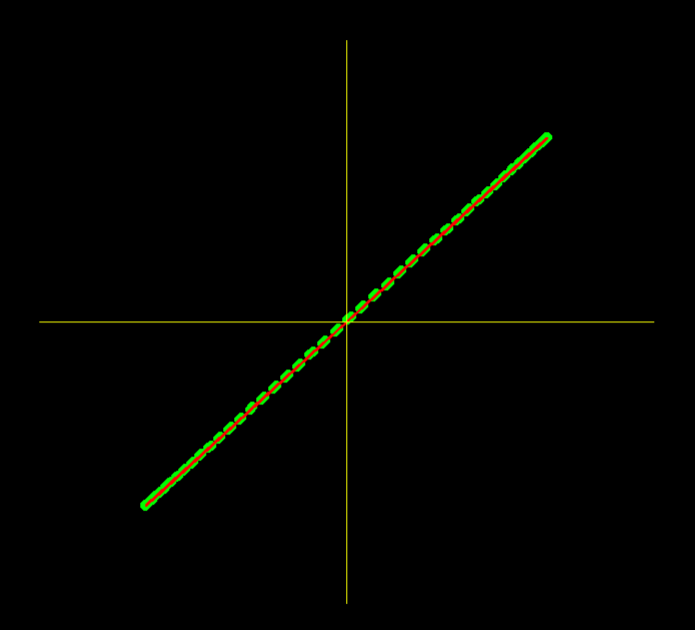
\includegraphics[scale=0.2]{22} \\
%
%
%\end{tabular}
%\end{center}
%\end{table}
%
%
%\smallpencil \hspace{0.2cm} \textcolor{col2}{\textbf{\textit{Eigenvectors and Eigenvalues}}} : Eigenvectors are those special vectors that, under the linear transformation defined by a matrix, remain within their own span, being scaled by a value, positive or negative depending on change of direction, called corresponding eigenvalues. \\
%	
%\hspace{0.5cm} In the \textcolor{col2}{\textbf{\textit{Scaling}}} example, observe that the vectors $\begin{bmatrix}
%1 \\ 0
%\end{bmatrix} $ and
%$ \begin{bmatrix}
%0 \\ 1
%\end{bmatrix} $ get transformed to 
%$\begin{bmatrix}
%1 \\ 0
%\end{bmatrix} $ and
%$ \begin{bmatrix}
%0 \\ 2
%\end{bmatrix} $ respectively but remain in their corresponding spans only. This makes 
%$\begin{bmatrix}
%1 \\ 0
%\end{bmatrix} $ and
%$ \begin{bmatrix}
%0 \\ 1
%\end{bmatrix} $ eigenvectors of 
%$ \begin{bmatrix} 
%      1 & 0 \\
%      0 & 2 
%    \end{bmatrix} $ with corresponding eigenvalues 1 and 2. \\
%    
%\faArrowAltCircleRight[regular] \textcolor{col1}{\textbf{\textit{Visualization}}} : 
%
%\begin{table}[!htbp]
%
%\begin{center}
%\begin{tabular}{cc}
%
%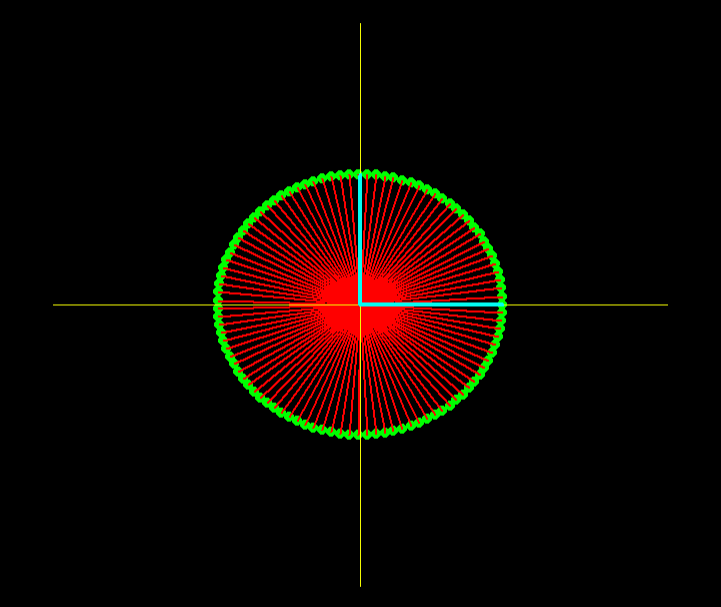
\includegraphics[scale=0.25]{23} &
%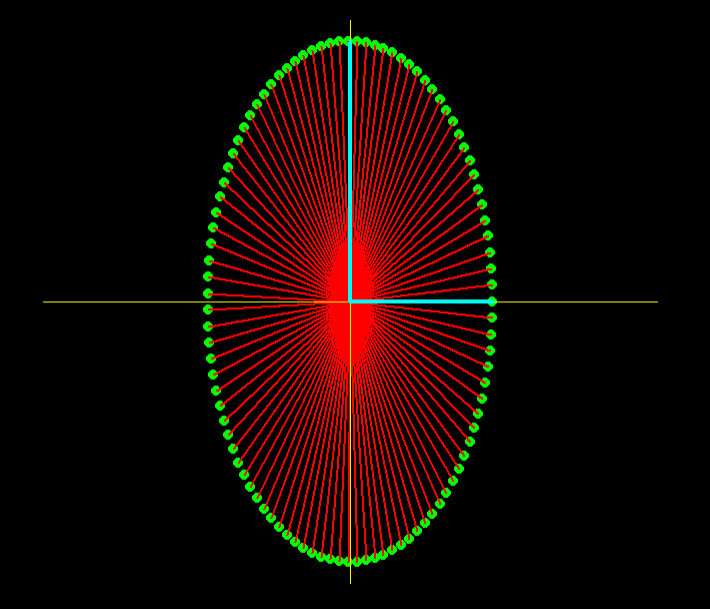
\includegraphics[scale=0.25]{24}
%
%\end{tabular}
%\end{center}
%
%\end{table}
%
%
%

\end{document}